\documentclass[12pt, a4paper]{article}

% ── Encoding & fonts ──
\usepackage[utf8]{inputenc}
\usepackage[T1]{fontenc}
\usepackage{mathptmx}          % Times for text + math
\usepackage[scaled=0.92]{helvet}
\usepackage{microtype}          % Optical margin alignment & font expansion

% ── Layout ──
\usepackage[margin=1in]{geometry}
\usepackage{setspace}
\usepackage{parskip}            % Paragraph spacing instead of indentation
\usepackage{enumitem}

% ── Visual polish ──
\usepackage[dvipsnames]{xcolor}
\usepackage{titlesec}
\usepackage{booktabs}
\usepackage{graphicx}
\usepackage{hyperref}
\hypersetup{
  colorlinks  = true,
  linkcolor   = NavyBlue,
  urlcolor    = NavyBlue,
  citecolor   = NavyBlue,
  pdfauthor   = {},
  pdftitle    = {AI-Assisted Summary Generation Methods},
}

% ── Heading styles ──
\definecolor{accent}{HTML}{1B3A5C}

\titleformat{\section}
  {\LARGE\bfseries\sffamily\color{accent}}
  {\thesection}{0em}{}
  [\vspace{2pt}{\color{accent!40}\titlerule[0.8pt]}]

\titleformat{\subsection}
  {\large\bfseries\sffamily\color{accent!85}}
  {\thesubsection}{0em}{}

\titlespacing*{\section}{0pt}{18pt}{10pt}
\titlespacing*{\subsection}{0pt}{14pt}{6pt}

% ── List styling ──
\setlist[enumerate]{
  topsep=4pt, itemsep=2pt, parsep=0pt,
  leftmargin=2em,
  label={\sffamily\small\color{accent}\arabic*.},
}

% ── Spacing ──
\doublespacing

% ═══════════════════════════════════════════════════
\begin{document}

\section*{AI-Assisted Summary Generation Methods}

This section describes the automated pipeline developed to generate structured best-practice guidance summaries from clinical trial documents using a large language model~(LLM). Figure~\ref{fig:pipeline} provides an end-to-end overview of the pipeline architecture.

\begin{figure}[ht]
  \centering
  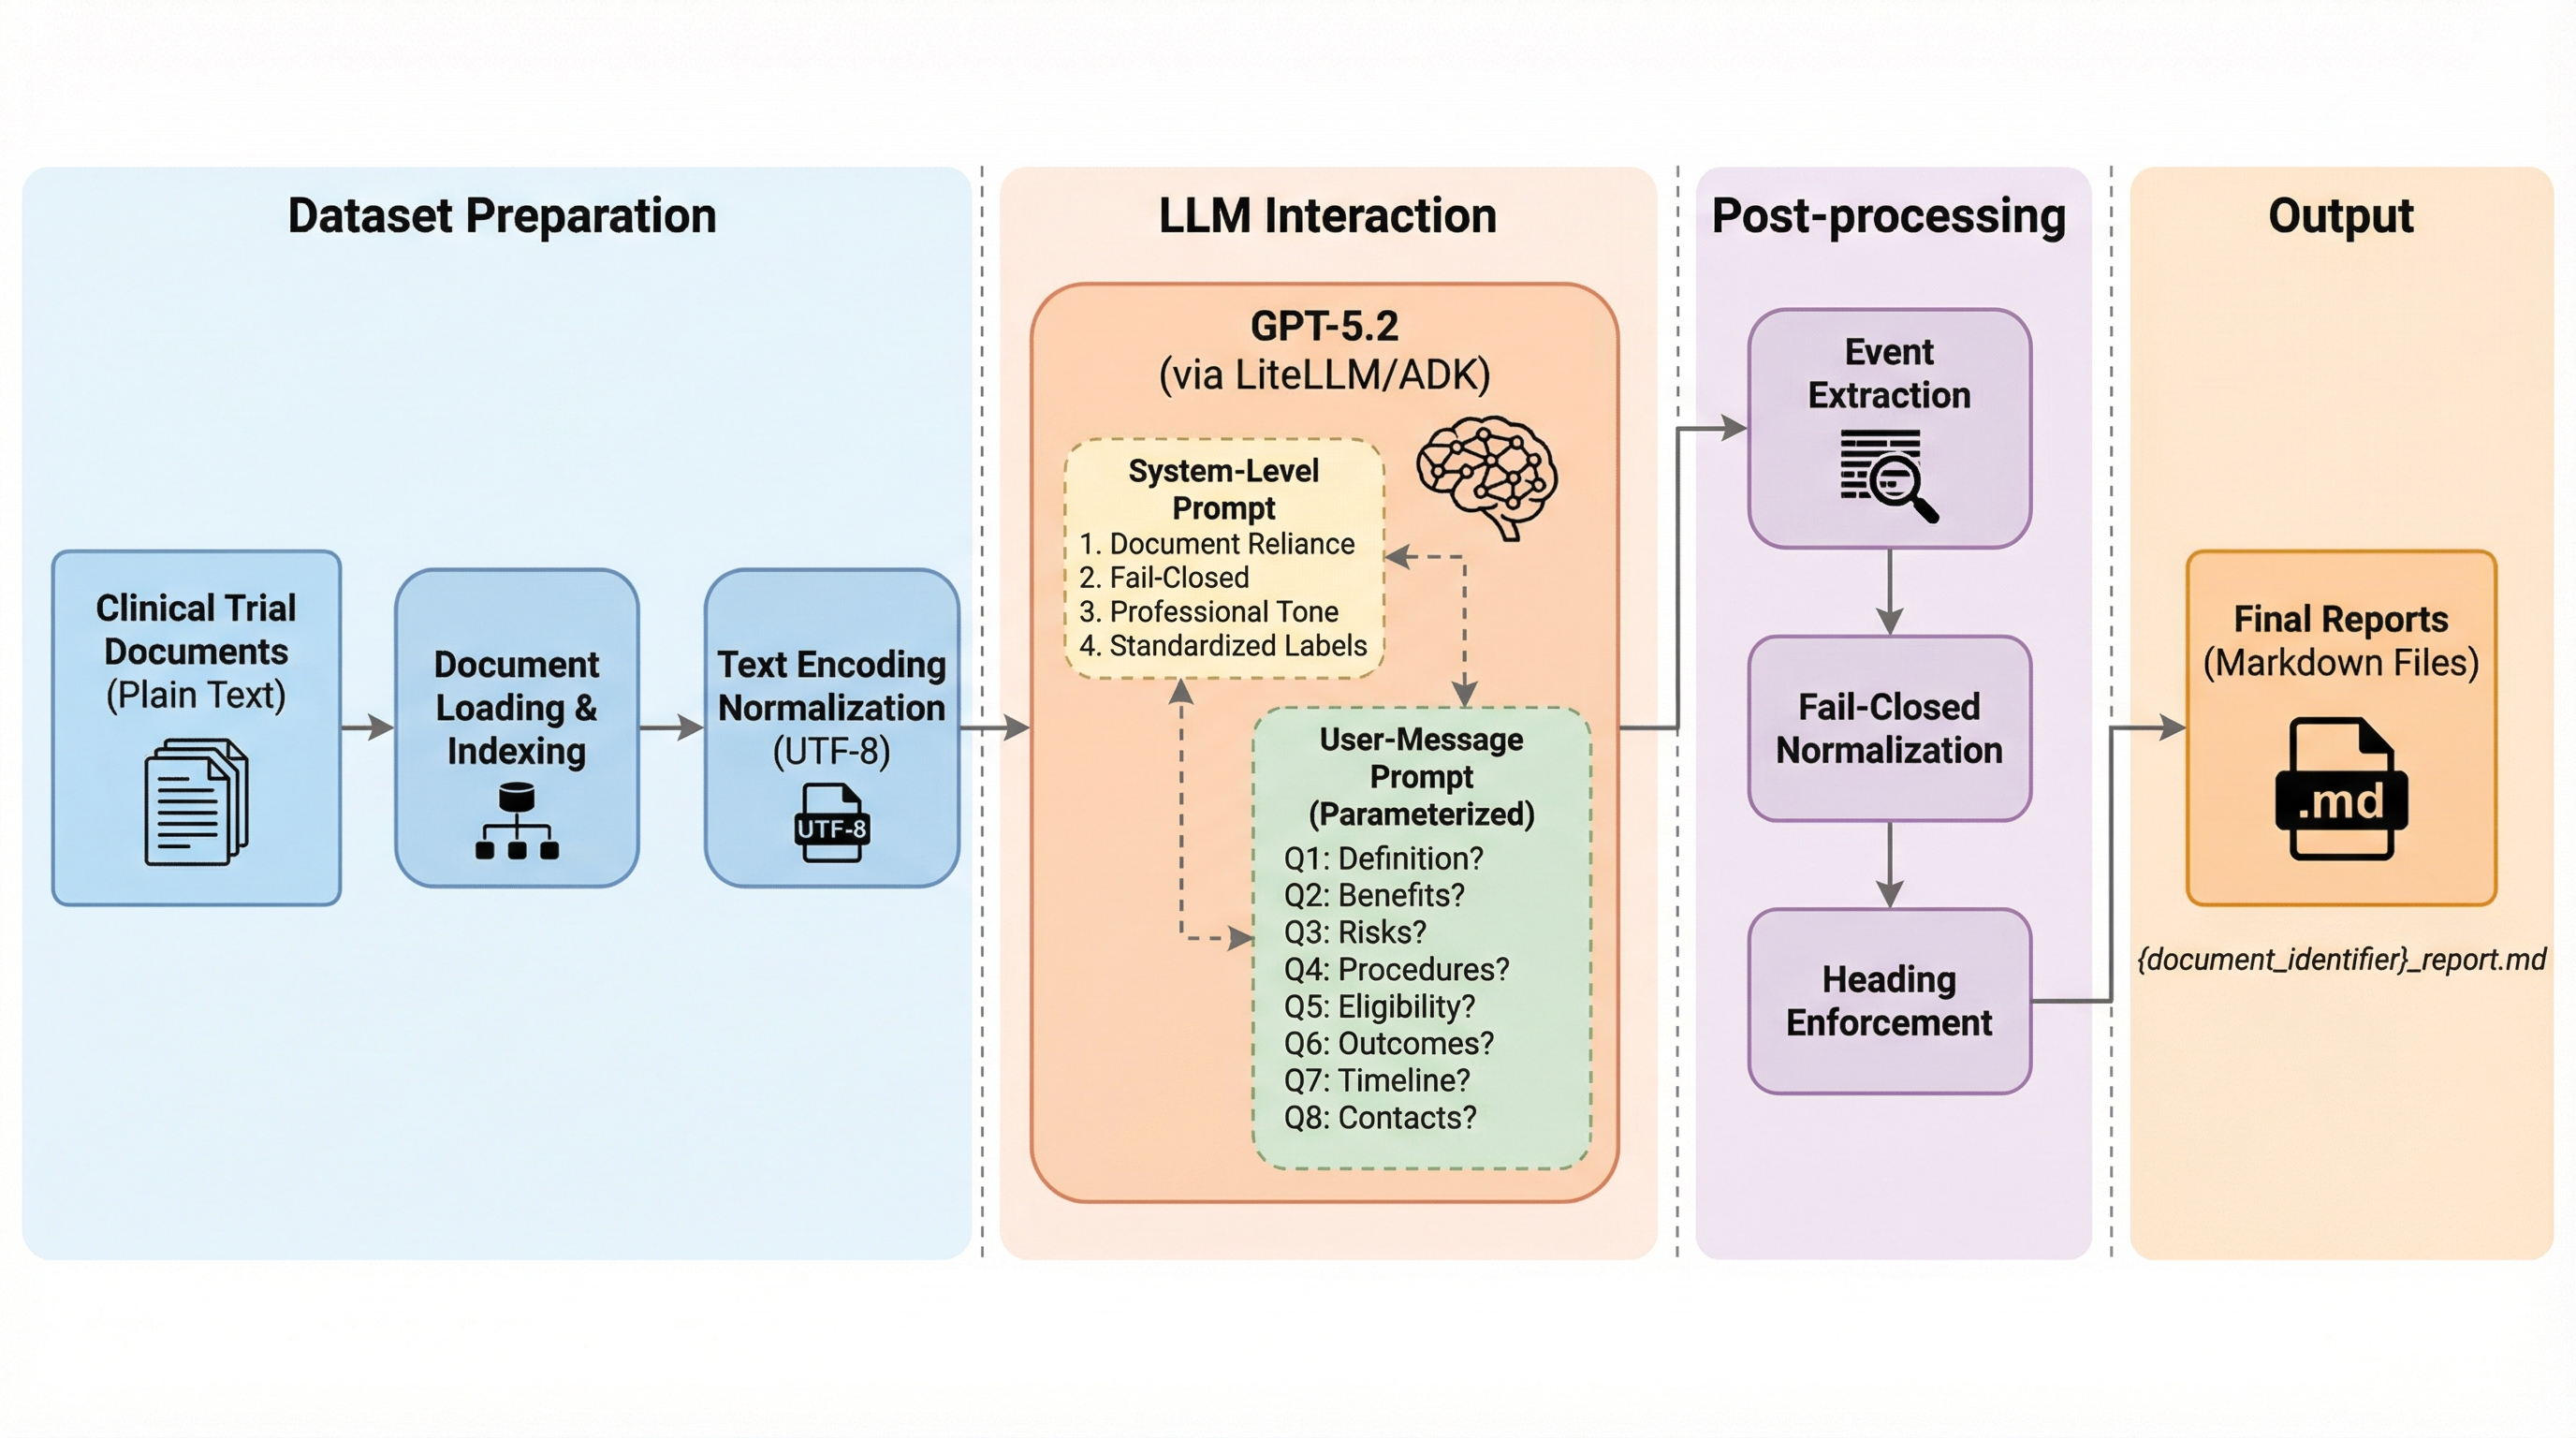
\includegraphics[width=\textwidth]{diagram.png}
  \caption{Overview of the AI-assisted summary generation pipeline. Clinical trial guidance documents are loaded and encoded (left), processed through GPT-5.2 via a two-tier prompting architecture (center), passed through three automated quality-control steps (right), and saved as structured Markdown reports (far right).}
  \label{fig:pipeline}
\end{figure}

% ── 1 ──
\subsection*{Dataset Preparation}

The input corpus consisted of clinical trial guidance documents in plain-text format. Each document addressed a distinct clinical trial practice, encompassing its definition, rationale, implementation protocols, evaluation criteria, and alternative approaches. Documents were loaded programmatically from a designated directory and indexed by filename identifier, enabling systematic tracking throughout the pipeline. Text encoding was normalized to UTF-8 with error-tolerant character handling to accommodate potential encoding artifacts. The source documents were sufficiently well-formed for direct model ingestion.

% ── 2 ──
\subsection*{Model Selection and Configuration}

Summary generation was performed using OpenAI's GPT-5.2, a large language model with strong long-context comprehension and instruction-following capabilities. The model was accessed through the LiteLLM abstraction layer integrated within the Google Agent Development Kit (ADK, version~$\geq$\,1.22.0), which provides an in-memory runner architecture for managing session state, message construction, and streamed response handling. Default inference parameters were used throughout, as output quality and structural consistency were governed by the prompting strategy detailed below. The LiteLLM integration additionally permits execution with alternative model providers, facilitating cross-model reproducibility assessment.

% ── 3 ──
\subsection*{Prompting Strategy}

A two-tier prompting architecture was designed to enforce consistent, document-grounded output across all processed documents.

The \emph{system-level} prompt established persistent behavioral constraints, specifying the model's role as a best-practice guidance report writer operating under four non-negotiable rules:
%
\begin{enumerate}[label=(\arabic*), nosep, leftmargin=2.4em]
  \item exclusive reliance on the provided document content, with no recourse to external knowledge, common-sense inference, or assumption;
  \item a fail-closed policy mandating the verbatim output ``Not found in document'' whenever the source material did not explicitly address a query or subsection;
  \item adoption of a professional, hierarchical guidance-report tone; and
  \item use of a standardized set of subsection labels---including ``Key messages,'' ``Definition and purpose,'' ``How to implement,'' and ``How to evaluate''---to ensure structural uniformity.
\end{enumerate}

At the \emph{user-message} level, a parameterized template was instantiated for each query, embedding the complete document text alongside a single question. Eight standardized questions were posed for every document:

\begin{enumerate}[nosep]
  \item What is the definition of this practice?
  \item Why is this practice beneficial or important?
  \item When should this practice be used?
  \item When is it justified to not use this practice?
  \item How should the correct methods be selected?
  \item How should the correct methods be implemented?
  \item How should the correct methods be evaluated?
  \item If it is justified not to use this practice, what should be done as an alternative?
\end{enumerate}

\noindent Each prompt directed the model to open its response with a standardized Markdown heading (e.g., \texttt{\#\#~Q1:~What is the definition of this practice?}) and to populate only those subsection labels applicable to the given question. This dual-layer design---persistent system constraints paired with per-question structural directives---constituted the primary mechanism for cross-document consistency.

% ── 4 ──
\subsection*{Generation Procedure and Quality Controls}

The processing pipeline was implemented as a fully asynchronous program. Documents were processed concurrently up to a configurable limit (default:~three) regulated by an asynchronous semaphore, while the eight questions within each document were posed sequentially. Sequential questioning preserved conversational session context within the ADK framework, enabling the model to accumulate topical awareness across questions for the same document. Each document was assigned an isolated in-memory session to prevent cross-document information leakage.

Three automated post-processing steps were applied to every model response:

\begin{enumerate}[nosep]
  \item \emph{Event extraction.}\enspace The ADK runner's streamed event objects were parsed and concatenated to reconstruct a single coherent text response.
  \item \emph{Fail-closed normalization.}\enspace Empty or null outputs were replaced with the canonical fallback string ``Not found in document,'' ensuring completeness.
  \item \emph{Heading enforcement.}\enspace The expected Markdown heading was verified and, if absent, prepended automatically to guarantee uniform report structure.
\end{enumerate}

\noindent Final reports were saved as individual Markdown files following the naming convention \texttt{\{document\_identifier\}\_report.md}. An overwrite-control flag permitted the pipeline to bypass previously completed documents on subsequent runs, eliminating redundant model invocations.

% ── 5 ──
\subsection*{Reproducibility Considerations}

The full pipeline---including all prompt texts, system instructions, and post-processing logic---was maintained under Git version control. Runtime configuration parameters (model identifier, directory paths, concurrency limits, and overwrite behavior) were externalized to an environment variable file, decoupling configuration from source code. Code quality was enforced through automated linting and formatting with Ruff, integrated via pre-commit hooks. While the deterministic components of the pipeline (prompt construction, post-processing, file output) are fully reproducible, large language model inference is inherently stochastic. The standardized prompting framework and structural post-processing serve to bound the practical impact of this variability on report structure and content coverage.

\end{document}
